\newcommand{\mriwidth}{2.2cm}
\newcommand{\gap}{0.00cm}

\definecolor{cases-default}{HTML}{EB5353}
\definecolor{controls-default}{HTML}{0079FF}
\definecolor{healthy-default}{HTML}{36AE7C}

\definecolor{baseline}{HTML}{FAEAB1}
\definecolor{preds}{HTML}{E5BA73}
\definecolor{maps}{HTML}{C58940}

\newcommand{\correlationplot}[4]{
    \definecolor{color0}{rgb}{0.62, 0.004, 0.259}
    \definecolor{color1}{rgb}{0.755, 0.154, 0.291}
    \definecolor{color2}{rgb}{0.866, 0.29, 0.298}
    \definecolor{color3}{rgb}{0.943, 0.406, 0.268}
    \definecolor{color4}{rgb}{0.975, 0.557, 0.323}
    \definecolor{color5}{rgb}{0.993, 0.709, 0.403}
    \definecolor{color6}{rgb}{0.995, 0.832, 0.506}
    \definecolor{color7}{rgb}{0.998, 0.926, 0.625}
    \definecolor{color8}{rgb}{0.998, 0.999, 0.746}
    \definecolor{color9}{rgb}{0.937, 0.975, 0.65}
    \definecolor{color10}{rgb}{0.838, 0.935, 0.609}
    \definecolor{color11}{rgb}{0.693, 0.876, 0.639}
    \definecolor{color12}{rgb}{0.527, 0.811, 0.645}
    \definecolor{color13}{rgb}{0.368, 0.725, 0.662}
    \definecolor{color14}{rgb}{0.24, 0.582, 0.721}
    \definecolor{color15}{rgb}{0.267, 0.441, 0.698}
    \definecolor{color16}{rgb}{0.369, 0.31, 0.635}

    \begin{tikzpicture}
        \begin{axis}[
            height=1.715 * \mriwidth,
            width=1.715 * \mriwidth,
            xmajorticks=false,
            ylabel=#3,
            ytick={0, 2, 4, 6, 8},
            yticklabels=#2,
            xmin=-1,
            xmax=17,
            ymin=0,
            ymax=9,
            every tick label/.append style={font=\tiny},
            ytick pos=left,
            scatter/classes={
                ADNI_EF={color0, draw=black},
                ADNI_MEM={color1, draw=black},
                CDCARE={color2, draw=black},
                CDCOMMUN={color3, draw=black},
                CDGLOBAL={color4, draw=black},
                CDHOME={color5, draw=black},
                CDJUDGE={color6, draw=black},
                CDMEMORY={color7, draw=black},
                CDORIENT={color8, draw=black},
                FAQTOTAL={color9, draw=black},
                GDTOTAL={color10, draw=black},
                MMSCORE={color11, draw=black},
                NPISCORE={color12, draw=black},
                PHC_EXF={color13, draw=black},
                PHC_LAN={color14, draw=black},
                PHC_MEM={color15, draw=black},
                PHC_VSP={color16, draw=black}
            },
            y label style={at={(-0.1,0.5)}},
            ymajorgrids=true,
            ytick style={draw=none},
            clip=false,
            grid style={draw=gray!20},
            axis line style={draw=gray!70}
        ]
            \addplot[
                only marks,
                scatter,
                scatter src=explicit symbolic
            ] table [
                col sep=comma,
                x=index,
                y=component_#1,
                meta=symptom
            ] {data/correlations.csv};
            \addplot[dashed,red, thick] coordinates {
                (-1, 2.76)
                (17, 2.76)
            };
            #4
        \end{axis}
    \end{tikzpicture}
}

\newsavebox{\firstcorrelations}
\sbox{\firstcorrelations}{%
    \correlationplot{0}{{0, 2, 4, 6, 8}}{\scriptsize{$-log_{10}(p)$}}{
        \node[] at (axis cs: 14, 6.19) {\tiny{PHC\_LAN}};
    }
}
\newsavebox{\secondcorrelations}
\sbox{\secondcorrelations}{%
    \correlationplot{1}{{,,}}{{}}{
        \node[] at (axis cs: 9, 3.74) {\tiny{FAQTOTAL}};
    }
}
\newsavebox{\thirdcorrelations}
\sbox{\thirdcorrelations}{%
    \correlationplot{2}{{,,}}{{}}{
        \node[] at (axis cs: 0, 6.44) {\tiny{ADNI\_EF}};
        \node[] at (axis cs: 13, 7.95) {\tiny{PHC\_EXF}};
    }
}
\newsavebox{\fourthcorrelations}
\sbox{\fourthcorrelations}{%
    \correlationplot{3}{{,,}}{{}}{
        \node[] at (axis cs: 0, 9.02) {\tiny{ADNI\_EF}};
        \node[] at (axis cs: 13, 8.75) {\tiny{PHC\_EXF}};
        \node[] at (axis cs: 14, 5.84) {\tiny{PHC\_LAN}};
        \node[] at (axis cs: 6, 5.18) {\tiny{CDJUDGE}};
        \node[] at (axis cs: 11, 3.99) {\tiny{MMSCORE}};
    }
}

\newcommand{\cognitivecorrelations}[1]{
    \begin{tikzpicture}
        \node[] at (-1.7, 1.2) {};
        \node[] at (8.7, -5) {};

        \node[] (first) at (0, 0) {
            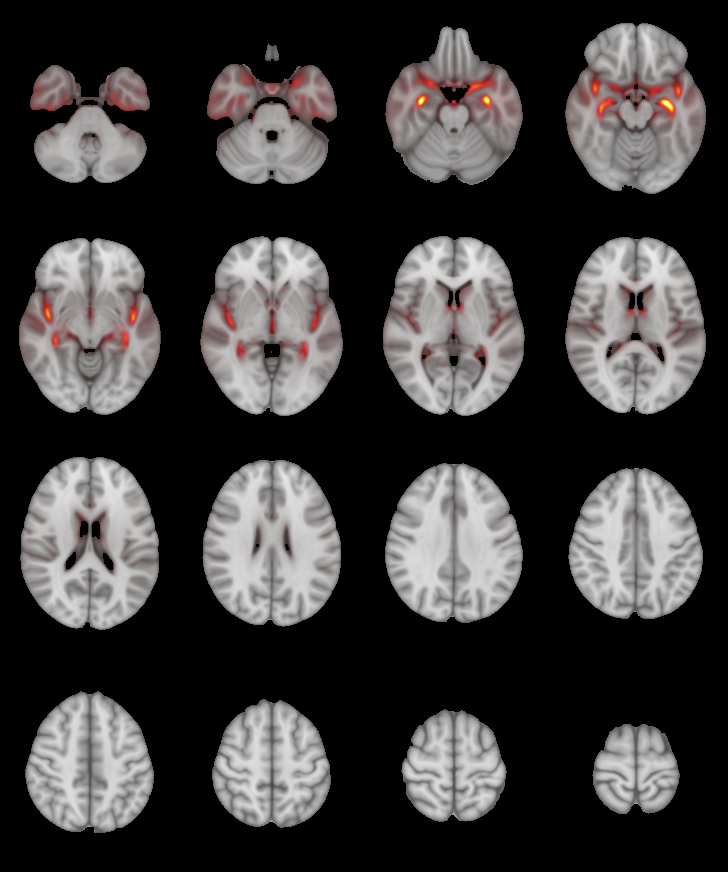
\includegraphics[
                width=\mriwidth,
                clip=true,
                trim = 192mm 232mm 0mm 0mm
            ]{data/components/component_0.png}
        };

        \node[anchor=west] (second) at ($ (first.east) + (\gap, 0) $) {
            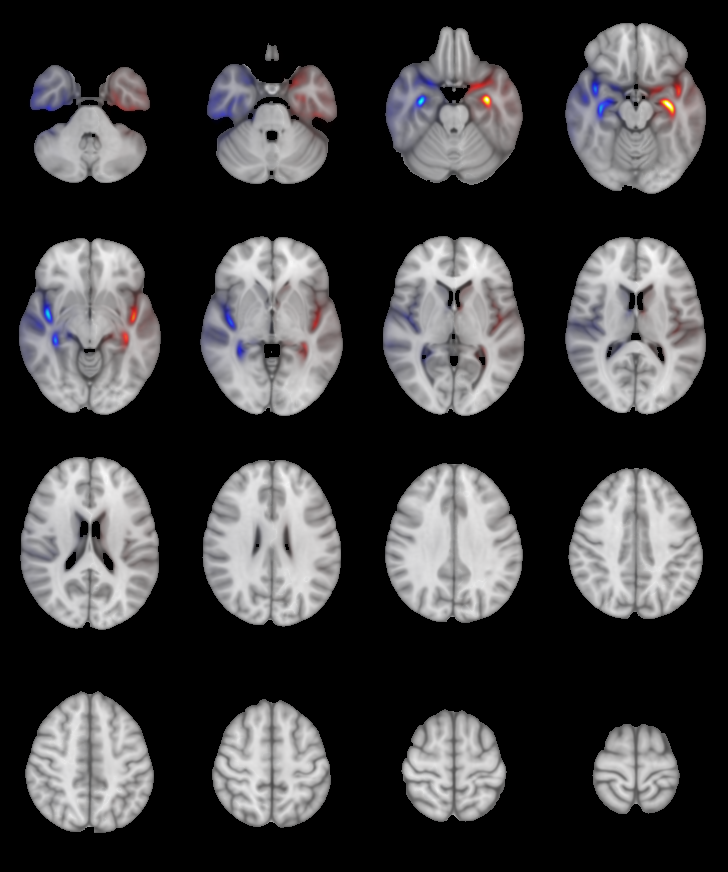
\includegraphics[
                width=\mriwidth,
                clip=true,
                trim = 192mm 232mm 0mm 0mm
            ]{data/components/component_1.png}
        };
        \node[anchor=west] (third) at ($ (second.east) + (\gap, 0) $) {
            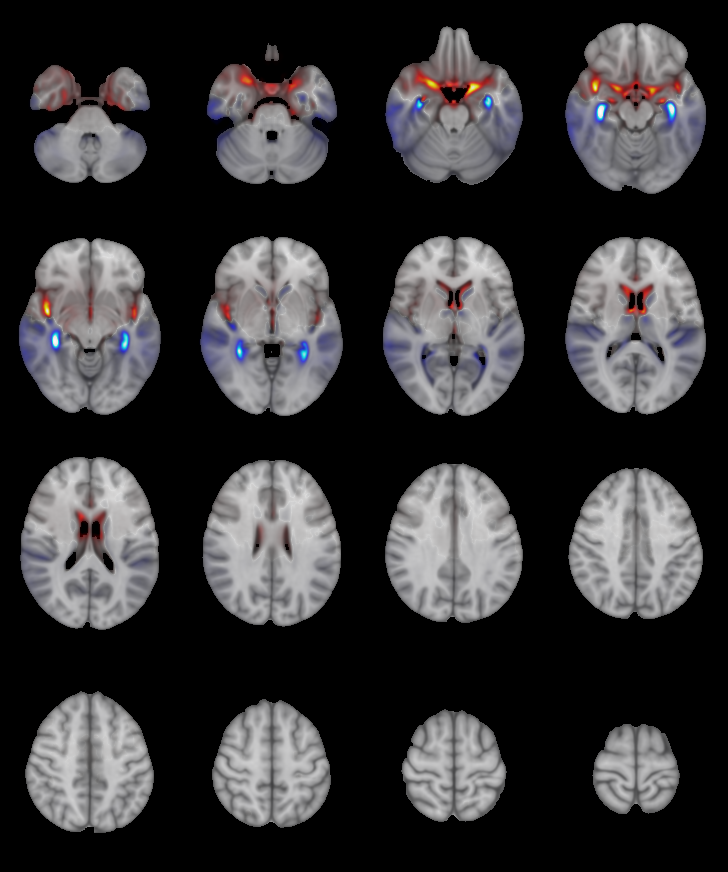
\includegraphics[
                width=\mriwidth,
                clip=true,
                trim = 192mm 232mm 0mm 0mm
            ]{data/components/component_2.png}
        };
        \node[anchor=west] (fourth) at ($ (third.east) + (\gap, 0) $) {
            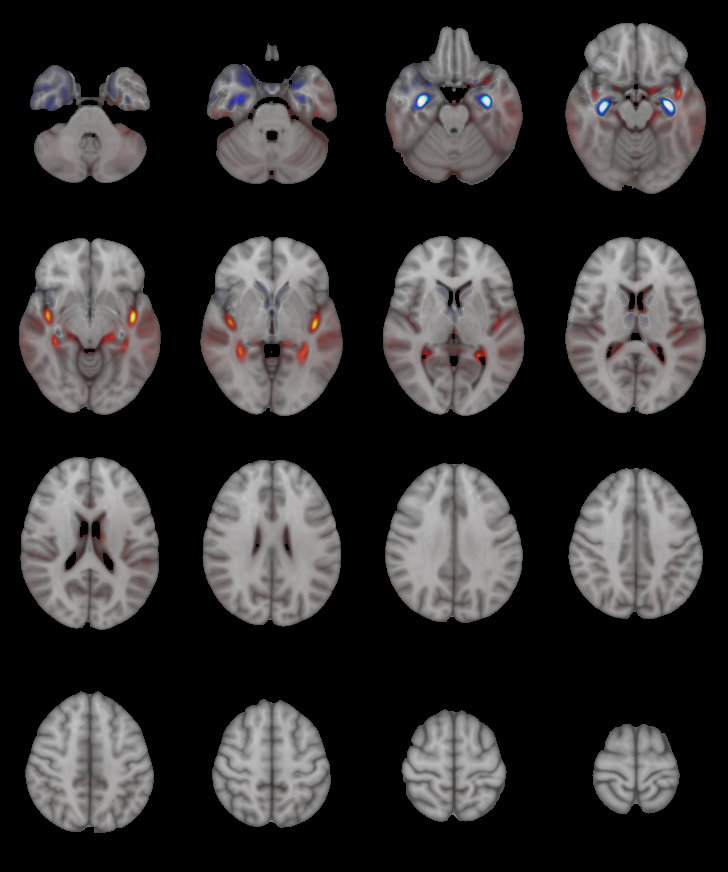
\includegraphics[
                width=\mriwidth,
                clip=true,
                trim = 192mm 232mm 0mm 0mm
            ]{data/components/component_3.png}
        };


        \ifnum#1>0
            \node[anchor=north west] (first-correlation) at ($ (first.south west) + (-0.5, -0.1) $) {
                \hspace{-2.3cm}
                \usebox{\firstcorrelations}
            };
        \fi
        \ifnum#1=2
            \node[anchor=north west] (second-correlation) at ($ (first-correlation.north east) - (0.297, 0) $) {
                \hspace{-2.4cm}
                \usebox{\secondcorrelations}
            };
            \node[anchor=north west] (third-correlation) at ($ (second-correlation.north east) - (0.255, 0) $) {
                \hspace{-2.4cm}
                \usebox{\thirdcorrelations}
            };
            \node[anchor=north west] (fourth-correlation) at ($ (third-correlation.north east) - (0.28, -0.21) $) {
                \hspace{-2.4cm}
                \usebox{\fourthcorrelations}
                \hspace{-0.6cm}
            };
        \fi
    \end{tikzpicture}
}

\newcommand{\prognostic}{
    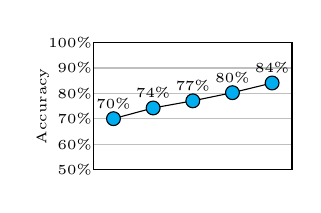
\begin{tikzpicture}
        \begin{axis}[
            height=3.2cm,
            width=4.1cm,
            xmajorticks=false,
            xmin=0.5,
            xmax=5.5,
            ymin=0.5,
            ymax=1,
            ylabel=\tiny{Accuracy},
            ymajorgrids=true,
            ytick={0.5, 0.6, 0.7, 0.8, 0.9, 1},
            yticklabels={50\%, 60\%, 70\%, 80\%, 90\%, 100\%},
            ytick style={draw=none},
            yticklabel style={font=\tiny, xshift=0.1cm},
            ylabel style={yshift=-0.25cm}
        ]
            \addplot[mark=*, draw=black, mark options={fill=cyan}, mark size=2.5pt] coordinates {
                (1, 0.701)
                (2, 0.743)
                (3, 0.771)
                (4, 0.803)
                (5, 0.841)
            };
            \node[anchor=south] at (axis cs: 1, 0.701) {\tiny{70\%}};
            \node[anchor=south] at (axis cs: 2, 0.743) {\tiny{74\%}};
            \node[anchor=south] at (axis cs: 3, 0.771) {\tiny{77\%}};
            \node[anchor=south] at (axis cs: 4, 0.803) {\tiny{80\%}};
            \node[anchor=south] at (axis cs: 5, 0.841) {\tiny{84\%}};
        \end{axis}
    \end{tikzpicture}
}

\newsavebox{\prognosticbox}
\sbox{\prognosticbox}{%
    \prognostic
}

\newcommand{\mciconcept}[1]{
    \begin{tikzpicture}
        \begin{axis}[
            height=0.7\textwidth,
            width=0.8\textwidth,
            xlabel={Age},
            ylabel={Cognitive function},
            ticks=none,
            axis x line=bottom,
            axis y line=left,
            y axis line style={-|},
            xmin=0,
            xmax=1.4,
            ymin=0,
            ymax=1,
            clip=false
        ]
            \addplot[draw=healthy-default, smooth, line width=4pt, opacity=0.5] coordinates {
                (0, 0.9)
                (0.25, 0.87)
                (0.5, 0.77)
                (0.6, 0.72)
                (0.8, 0.63)
                (0.9, 0.72)
                (1.4, 0.67)
            };
            \addplot[draw=controls-default, smooth, line width=4pt, opacity=0.5] coordinates {
                (0, 0.9)
                (0.25, 0.87)
                (0.5, 0.77)
                (0.6, 0.72)
                (0.8, 0.63)
                (0.9, 0.61)
                (1.4, 0.54)
            };
            \addplot[draw=cases-default, smooth, line width=4pt, opacity=0.5] coordinates {
                (0, 0.9)
                (0.25, 0.87)
                (0.5, 0.77)
                (0.6, 0.72)
                (0.8, 0.625)
                (1.1, 0.48)
                (1.4, 0.3)
            };
            \addplot[dashed] coordinates {
                (0, 0.65)
                (1.4, 0.65)
            };
            \addplot[dashed] coordinates {
                (0, 0.4)
                (1.4, 0.4)
            };
            \node[anchor=south west] at (axis cs: 0, 0.64) {\footnotesize{Normal cognition}};
            \node[anchor=north west] at (axis cs: 0, 0.66) {\footnotesize{Mild cognitive impairment}};
            \node[anchor=north west] at (axis cs: 0, 0.41) {\footnotesize{Dementia}};

            \node[anchor=west] at (axis cs: 1.4, 0.67) {\textcolor{healthy-default}{\footnotesize{Improving (n=80)}}};
            \node[anchor=west] at (axis cs: 1.4, 0.53) {\textcolor{controls-default}{\footnotesize{Stable (n=754)}}};
            \node[anchor=west] at (axis cs: 1.4, 0.3) {\textcolor{cases-default}{\footnotesize{Progressive (n=354)}}};

            \ifnum#1>0
                \draw[-stealth, red, thick] (axis cs: 0.8, 0.8) -- (axis cs: 0.8, 0.67);
                \node[anchor=south] at (axis cs: 0.8, 0.8) {\textcolor{red}{\footnotesize{t}}};
            \fi

            \ifnum#1>1
                \draw[densely dotted] (axis cs: 0.9, 0.8) -- (axis cs: 0.9, 0.3);
                \draw[densely dotted] (axis cs: 1, 0.8) -- (axis cs: 1, 0.3);
                \draw[densely dotted] (axis cs: 1.1, 0.8) -- (axis cs: 1.1, 0.3);
                \draw[densely dotted] (axis cs: 1.2, 0.8) -- (axis cs: 1.2, 0.3);
                \draw[densely dotted] (axis cs: 1.3, 0.8) -- (axis cs: 1.3, 0.3);
                \node[anchor=south] at (axis cs: 0.9, 0.8) {\footnotesize{t+1}};
                \node[anchor=south] at (axis cs: 1, 0.8) {\footnotesize{t+2}};
                \node[anchor=south] at (axis cs: 1.1, 0.8) {\footnotesize{t+3}};
                \node[anchor=south] at (axis cs: 1.2, 0.8) {\footnotesize{t+4}};
                \node[anchor=south] at (axis cs: 1.3, 0.8) {\footnotesize{t+5}};
            \fi

            \ifnum#1=3
                \node[] at (axis cs: 1.015, 0.162) {
                    \usebox{\prognosticbox}
                };
            \fi

        \end{axis}
    \end{tikzpicture}
}

\begin{frame}{Explainable AI and dementia}
    \begin{tikzpicture}
        \node[] at (-5.25, -3.5) {};
        \node[] at (5.25, 3.5) {};

        \only<1-2>{
            \node[label={[text depth=0]above:Explainable AI}] at (-2.25, 0) {
				
\includegraphics[width=0.31\textwidth]{data/dementia.png}
			};
        }
        \only<2>{
			\node[label={[text depth=0]above:Human researchers}] at (2.25, 0) {
				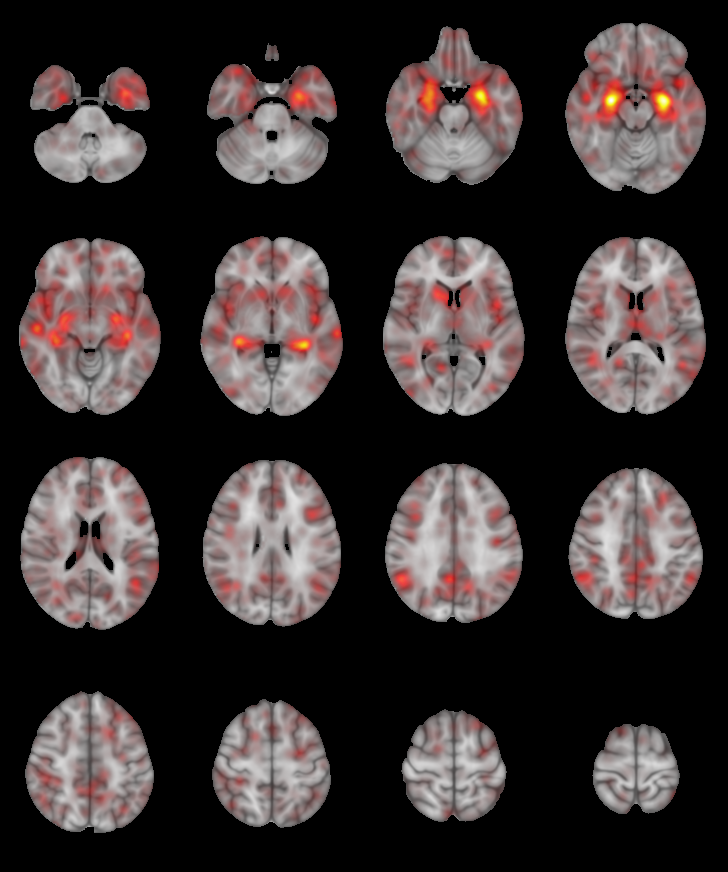
\includegraphics[width=0.31\textwidth]{data/ALE.png}
			};
        }

        \only<3>{
            \node[text width=10cm, font=\scriptsize, align=center] at (0, 0) {
                \renewcommand{\arraystretch}{1.2}
                \begin{tabular}{|>{\centering\arraybackslash}m{2.55cm}|>{\centering\arraybackslash}m{1.45cm}|>{\centering\arraybackslash}m{1.3cm}|>{\centering\arraybackslash}m{2.9cm}|}
                    \hline
                    \textbf{Test battery}&\textbf{Domain}&\textbf{Name}&\textbf{Description}\\
                    \hline
                    Functional Activities Questionnaire&&FAQTOTAL&Measures instrumental activities from everyday life\\
                    \hline
                    ADSP Phenotype Harmonization Consortium&Language&PHC\_LAN&Composite language score\\
                    \hline
                    UW - Neuropsych Summary Scores&Executive functioning&ADNI\_EF&Composite score for executive functioning\\
                    \hline
                    UW - Neuropsych Summary Scores&Memory&ADNI\_MEM&Composite score for memory\\
                    \hline
                \end{tabular}
                \textbf{\vdots}
            };
        }
        \only<4>{
            \node[] at (0.3, 0) {
                \cognitivecorrelations{0}
            };
        }
        \only<5>{
            \node[] at (0.3, 0) {
                \cognitivecorrelations{1}
            };
        }
        \only<6>{
            \node[] at (0.3, 0) {
                \cognitivecorrelations{2}
            };
        }
        \only<7>{
            \node[] at (0, 0) {
                \mciconcept{0}
            };
        }
        \only<8>{
            \node[] at (0, 0) {
                \mciconcept{1}
            };
        }
        \only<9>{
            \node[] at (0, 0) {
                \mciconcept{2}
            };
        }
        \only<10>{
            \node[] at (0, 0) {
                \mciconcept{3}
            };
        }
    \end{tikzpicture}
\end{frame}
